\section{Experimental evaluation}\label{sec:eval}
In this section, we will display results of our experiments. First, we will establish baseline performance results for Zookeeper. These results will aid us in reasoning for following experiments. Next, we implemented previously discussed synchronization primitives, namely Test-and-set, queues, and their asynchronous counterparts. We perform several experiments with them to test their performance on various conditions. \note{if we did application subsection then add here}.
%In this section we establish a baseline performance for zookeeper on our
%testbed and then provide latency and throughput numbers for the selected
%synchronization primitives.

%Baseline numbers for zookeeper are obtained using smoketest [ref]. We explore
%the performance of test-and-set and queue locks implemented in Java.

%We first set up zookeeper with 1, 3 and 5 processes on a single machine and
%observe the experiments. Then, we fan out the processes to distict machines and
%measure the impact of added network latency on basic operations and the
%synchronization primitives. \note{Finally, we repeat the experiments on
%geographically distributed nodes in EC2}


%\subsection{Test bed}
%\note{multiple physical machines}
%The testbed consists of 5 quad-core Xeon \note{type and clock} machines with commodity 500GB 7.2k rpm disks. They are interconnected with 1Gbps Ethernet on a single switch. \note{should we move this and expand it to section 2? I think a figure showing connections and showing that hamilton is connected to them would be a nice display.}
%\note{Average RTT for pings is (ping lat)
%Average network throughput is (throughput=). this for inter-cluster and cluster to hamilton.}

%\begin{figure}[h]
%\centering
%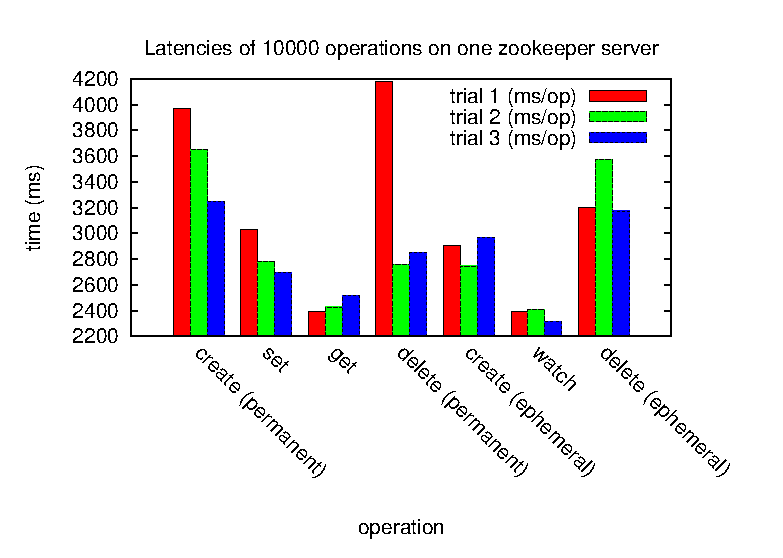
\includegraphics[scale=0.75]{img/1_machine_1_server.eps}
%\caption{}
%\label{fig:1machine_1server_latency}
%\end{figure}

\subsection{Baseline performance}
\note{smoketest, zk-latencies and baseline} In this section we will perform experiments to establish a baseline for later experiments. We would like to establish limits on the system. These limits represent workloads and environment conditions that will saturate the system. Workload is represented by the number of clients, number of requests per second, and the type of requests. Environment conditions are the number of zookeeper servers and condition of links connecting them.

%We begin by measuring the latencies of basic Zookeeper operations. Our first experiment is performed on one machine having one zookeeper server. This means that there are no communication overhead for consensus. One client issues 10000 calls of each tested operations and we report the total time required to complete them. The results as shown in Figure~\ref{fig:1machine_1server_latency}\footnote{These results are obtained from a different server than those in next figures. It will be changed in the final draft for consistency} for asynchronous versions of operations. We report detailed results of three trials to show the variability of zookeeper behavior. In the figure we report latencies of adding and deleting in both cases, permanent and ephemeral. Creating a permanent node incur more bandwidth than creating a ephemeral node. On the other hand, deleting an ephemeral node incur more bandwidth than deleting permanent nodes (except for first trial that is due variability of behavior). Other observations are that set operations are more expensive than get operations, as expected. Also, the implementation of watches is efficient.

%\begin{figure}[h]
%\centering
%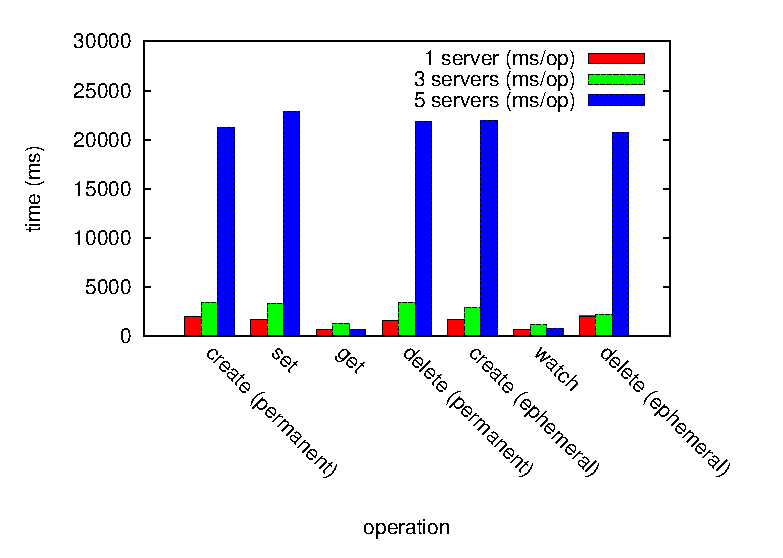
\includegraphics[scale=0.75]{img/1_machine_diff_cpu.eps}
%\caption{Latencies of 10000 operations on various number of zookeeper servers with asynchronous operations on one machines}
%\label{fig:1machine_diffcpu_latency}
%\end{figure}

%\begin{figure}[h]
%\centering
%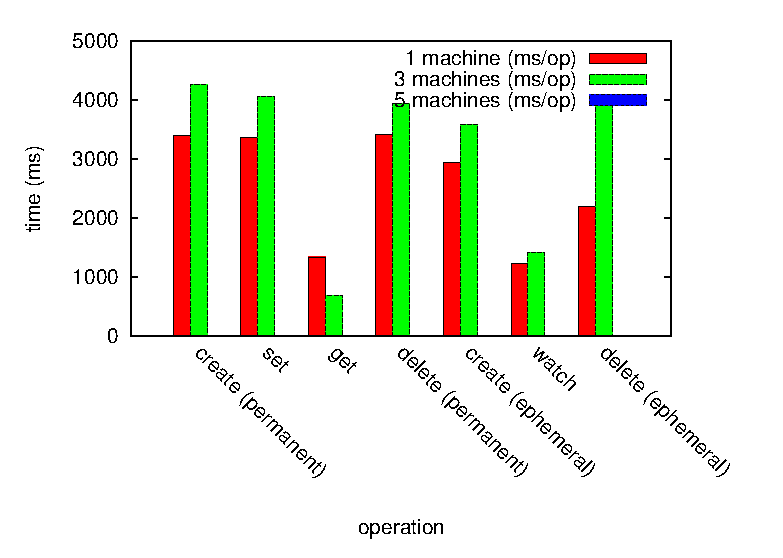
\includegraphics[scale=0.75]{img/1_machine_diff_machines.eps}
%\caption{Latencies of 10000 operations on three zookeeper server with asynchronous operations while changing number of machines}
%\label{fig:1machine_diffservers}
%\end{figure}

%Our next set of results are done to test the effect of increasing the number of Zookeeper servers. Results are shown in Figure~\ref{fig:1machine_diffcpu_latency}. These results are collected when running all servers in one machine. Thus, communication overhead between servers is minimal. As shown in the figure, increasing the number of servers to five servers have a dramatic effect on latency.
%In Figure~\ref{fig:1machine_diffservers} we show results of fanning out Zookeeper servers. We test the performance of three Zookeeper servers running on different number of machines, namely 1, 2, and 3 servers\footnote{results for five servers are not ready yet}. \ldots

\begin{figure}[h]
\centering
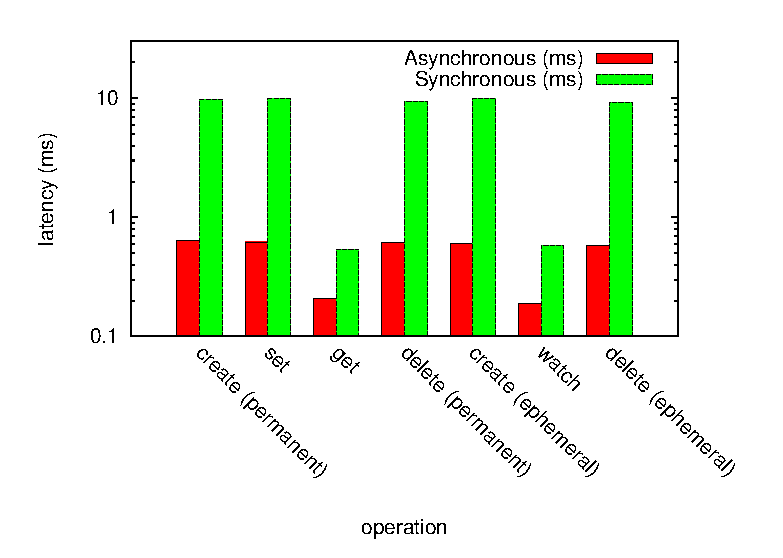
\includegraphics[scale=0.75]{img/ops_latencies_logscale.eps}
\caption{Zookeeper basic operations latencies for a cluster of five servers}
\label{fig:ops_latencies}
\end{figure}

Our first experiment test basic Zookeeper operations' latencies. We test both synchronous and asynchronous versions of these operations. For testing we use zk-smoketest\footnote{https://github.com/phunt/zk-smoketest}. Each operation is run for a thousand time and we report average latency. Results are shown in Figure~\ref{fig:ops_latencies}. Synchronous operations block until the operation is performed, thus giving an indication on the total time taken to perform the actual operation. Asynchronous operations on the other hand do not block. The figure shown that synchronous operations takes more than ten times the latency of asynchronous operations for \emph{put} operations, and around double the latency for \emph{get} operations. \note{define put and get operation classes either here or before (section II)}. 

\subsection{synchronization primitives}
\note{test test-and-set and queues (as in paper: reactive synchronization}

\subsection{application performance}
\note{map reduce. effect of adding machines, effect of adding zookeeper servers.}

